\section{Resultados y Análisis}
\subsection{Software}
\begin{frame}[t]
\frametitle{Resultados y Análisis}
\framesubtitle{Aplicación Web}
\begin{columns}[t]
	\column[t]{0.5\linewidth}
	\begin{figure}[!]
		\centering
		\caption{Vista Usuario Administrador. [Imagen Propia]}
		\label{fig:adminview}
		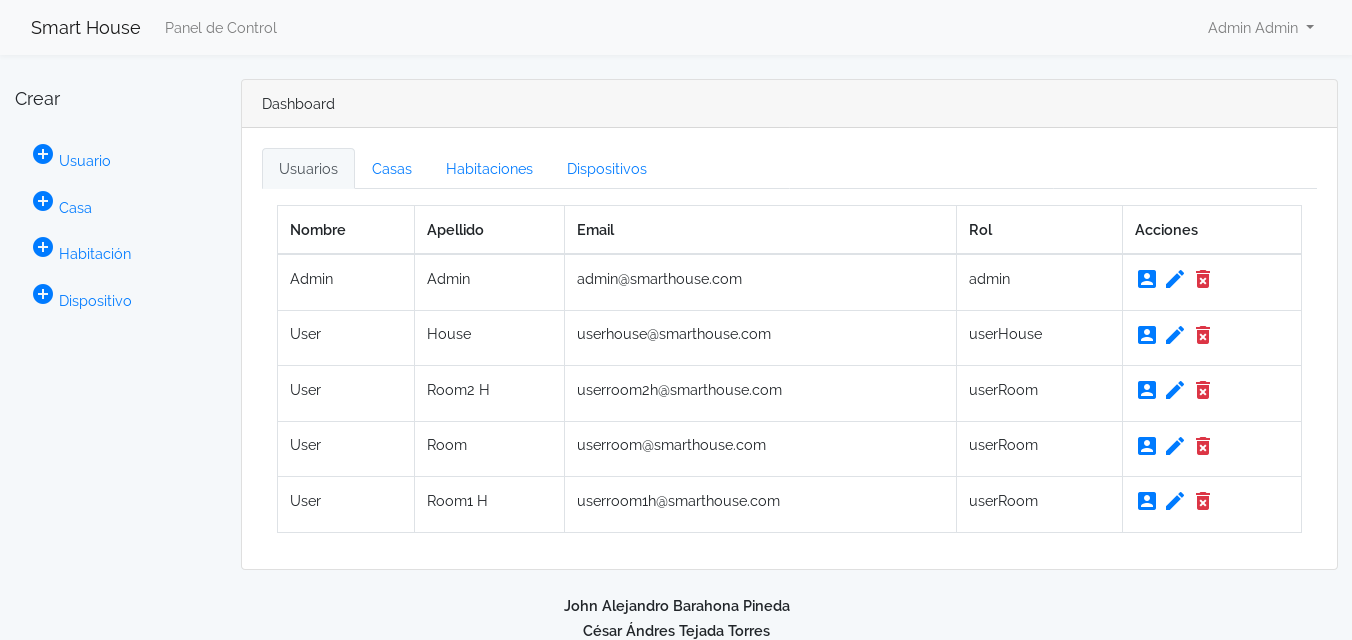
\includegraphics[width=\linewidth]{Imagenes/Admin_view}
	\end{figure}
	
	\column[t]{0.5\linewidth}
	\begin{figure}[!]
		\centering
		\caption{Vista Usuario de Casa. [Imagen Propia]}
		\label{fig:houseview}
		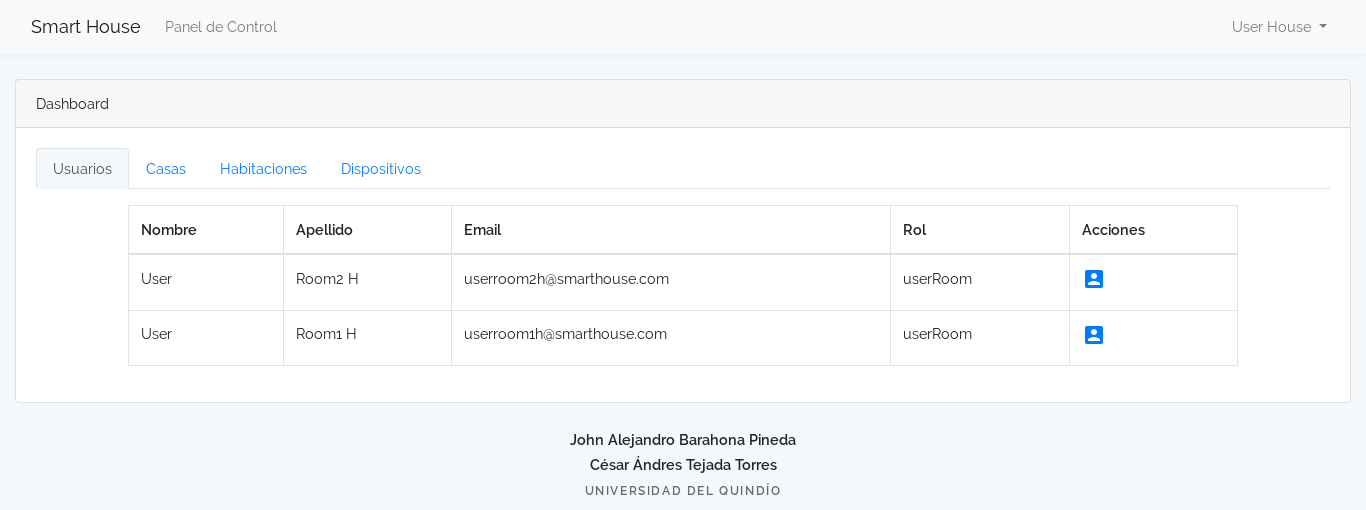
\includegraphics[width=\linewidth]{Imagenes/UserH_view}
	\end{figure}

\end{columns}
\end{frame}

\begin{frame}[t]
\frametitle{Resultados y Análisis}
\framesubtitle{Aplicación Web}
\begin{columns}
	\column[t]{0.5\linewidth}
	\begin{figure}[!]
		\centering
		\caption{Vistas de Usuario Habitación [Imagen Propia]}
		\label{fig:userview}
		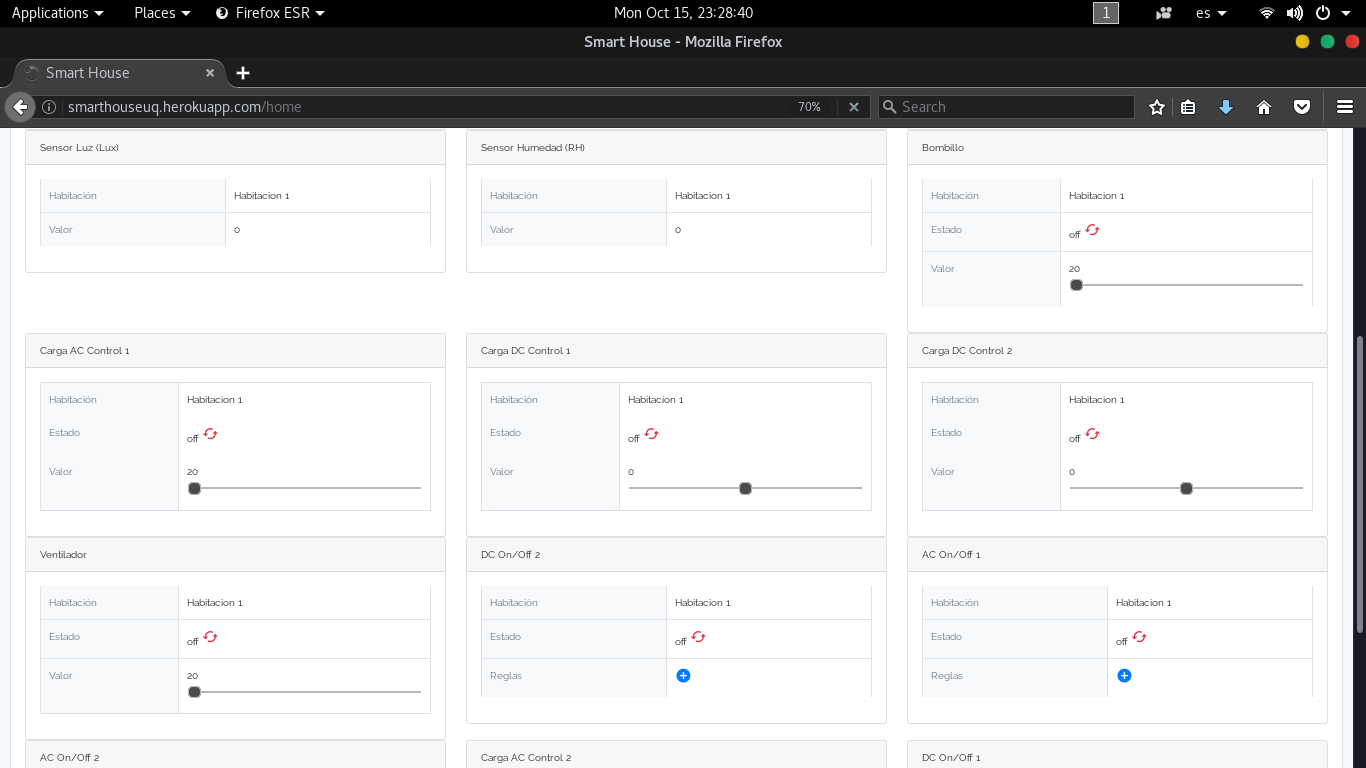
\includegraphics[width=\linewidth]{Imagenes/UserR_view}
	\end{figure}

	\column[t]{0.5\linewidth}
	\begin{figure}[!]
		\centering
		\caption{Vista para añadir reglas [Imagen Propia]}
		\label{fig:rulesview}
		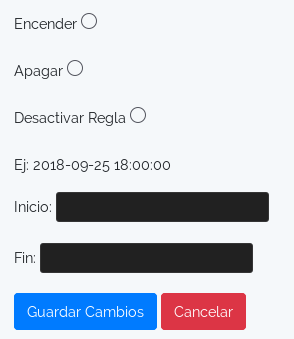
\includegraphics[width=0.5\linewidth]{Imagenes/rules_view}
	\end{figure}
\end{columns}
\end{frame}

\subsubsection{Base de Datos}
\begin{frame}
\frametitle{Resultados y Análisis}
\framesubtitle{Software | \emph{Base de Datos}}
\begin{figure}[H]
\centering
\caption{Base de datos SmartHouse [Imagen Propia]}
\label{fig:db}
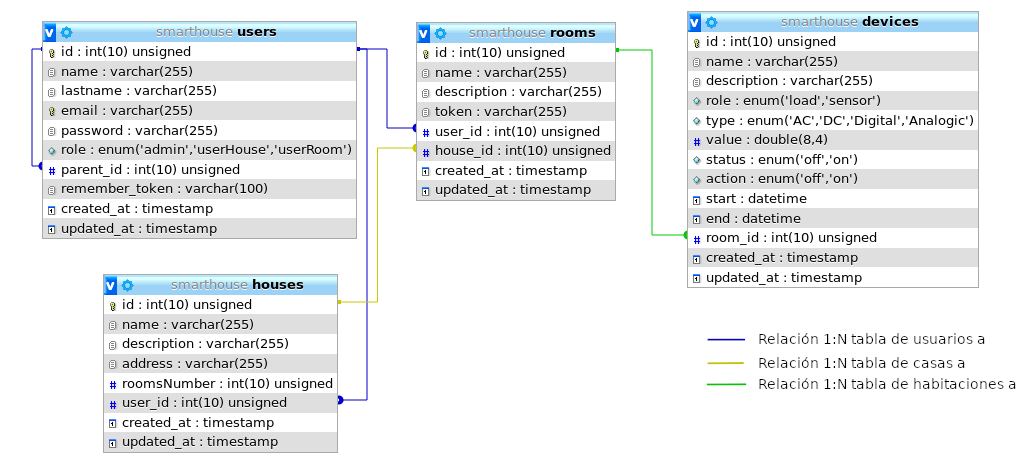
\includegraphics[width=0.75\linewidth]{Imagenes/DB}
\end{figure}

\end{frame}


\subsection{Firmware}
\begin{frame}
\frametitle{Resultados y Análisis}
\framesubtitle{Firmware}
%Modificar esta imagen, pero es parecida al producto final, falta el usuario y colocar logos de los productos usados WiFi ESP32 etc...

%Añadir tabla
\begin{wrapfigure}{r}{0.5\linewidth}
	\centering
	\caption{Conexión a Internet vía Wi-Fi ESP32 [Imagen Propia]}
	\label{fig:conexion}
	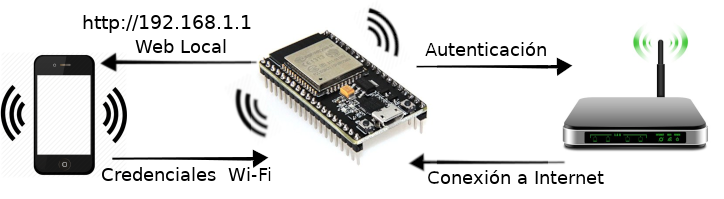
\includegraphics[width=\linewidth]{Imagenes/conexion}
\end{wrapfigure}
Falta
\end{frame}

\subsection{Hardware}
\begin{frame}[t]
\frametitle{Resultados y Análisis}
\framesubtitle{Hardware}
%Cambiar Imagen

\begin{figure}[t]
	\centering
	\caption{Tarjeta SmartHouse [Imagen Propia]}
	\label{fig:tarjeta}
	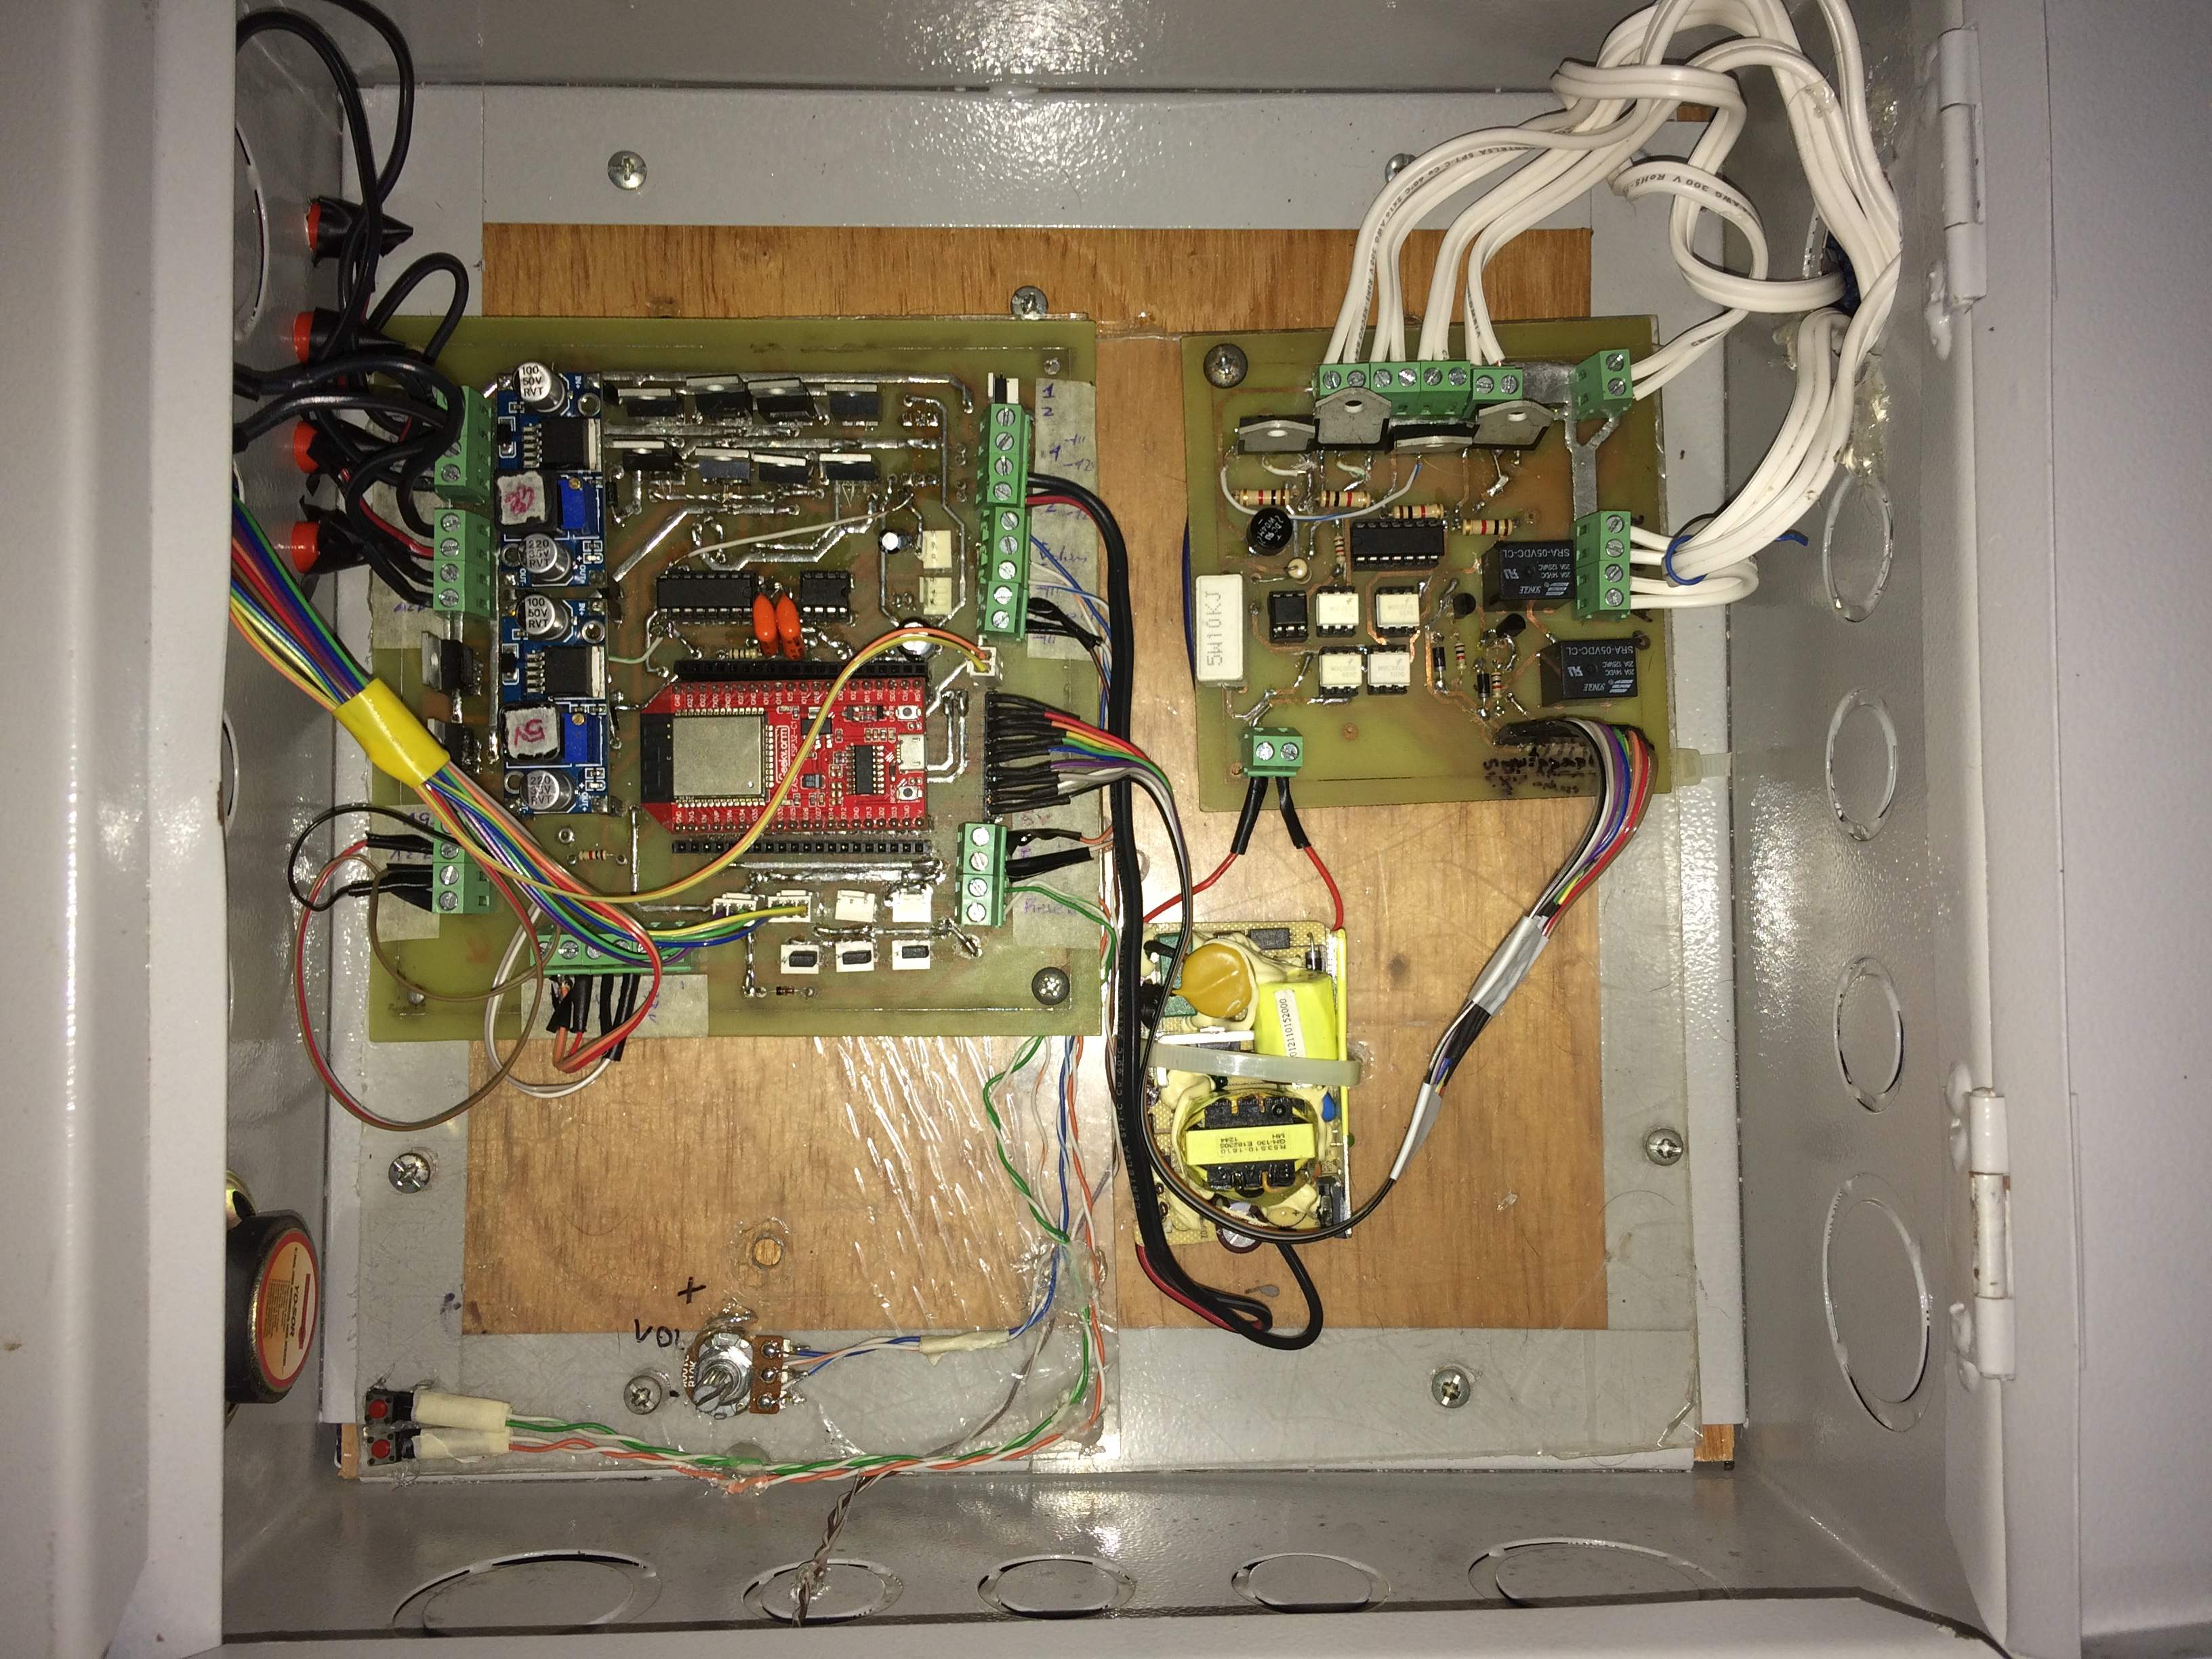
\includegraphics[width=\linewidth]{Imagenes/Tarjeta}
\end{figure}
\end{frame}



\subsection{Prueba Beta Cerrada}
\begin{frame}[t]
\frametitle{Resultados y Análisis}
\framesubtitle{Prueba Beta Cerrada}
\footnotesize %Colocar el enfoque de las preguntas para dar claridad.
La prueba se realiza a quince personas, entre los cuales algunos son estudiantes de ingería electrónica y personas ajenas a este tipo de escenarios, los resultados de la prueba se consignan en la tabla \ref{table:enc}.

\begin{table}[H]
	\begin{center}
		\caption{Resultados por pregunta.}
		\label{table:enc}
		\begin{tabular}{|c|c|}
			\hline 
			\textbf{Número de la Pregunta} & \textbf{Promedio} \\ 
			\hline 
			1 & 4.5\\ 
			\hline 
			2 & 4.8\\ 
			\hline 
			3 & 4.5\\ 
			\hline 
			4 & 5.0\\ 
			\hline 
			5 & 4.9\\ 
			\hline 
			6 & 4.9\\ 
			\hline 
			7 & 4.3\\ 
			\hline 
			8 & 4.3\\ 
			\hline 
			9 & 4.8\\ 
			\hline 
			\textbf{Total} & \textbf{4.7}\\ 
			\hline 
		\end{tabular} 
	\end{center}
\end{table}

En resumen, la aplicación recibe una calificación de 4.7, por lo tanto se puede decir que las funcionalidades requeridas están programadas de una manera adecuada y simple para que el usuario disponga de ellas, pero es posible mejorarlas con el objetivo de que sean mucho más intuitivas para el usuario y que no se le presenten dudas al momento de usarla. Conforme a las observaciones obtenidas durante la prueba se han modificado algunas partes del sistema, que no tienen un impacto significativo sobre los objetivos ni alcances propuesto en este trabajo.\\

\end{frame}